
\section{CRT cuts: CRT Veto and Distance Tagger}\label{sec:Cuts}
In this section, we define the  CRT Veto and Distance Tagger cuts used in the preselection.
\subsection{CRT Veto}\label{sec:VetoCuts}
On average, only one in six events passing the MicroBooNE common optical filter is associated to beam-induced activity; the remaining events are triggered by activity that originates outside the TPC: either external beam induced activity or cosmic rays. Given the $\mathcal{O}(10)$ CR muons in each drift window, this equates to a starting signal-to-background of $\sim 1 : 60$. The scope of the CRT Veto is to reduce these backgrounds by looking at CRT activity in time with the beam window. 
The CRT veto looks for a coincidence in time between the scintillation light recorded in time with the 1.6 $\mu$s beam-spill (beam-flash) and a CRT hit: if a CRT hit occurs within a 1 $\mu s$ of the beam flash, the event is rejected. For this coincidence, only CRT hits with PE $>$ 100 pe are considered; we do not apply a constraint on the position of the flash nor on the position of the CRT hit. The pe distribution of CRT hits for BNB External data and CORSIKA simulation is shown in figure \ref{fig:CRTPe};  simulation has been tuned to replicate the CRT response for minimum ionizing particles. Neutrons are mostly responsible for the low pe activity in the CRT. Even if this activity is not well modeled in the CRT simulation, we believe the pe threshold choice makes it unlikely for neutrons to generate a CRT hit and we are currently working to demonstrate this with data. 

A back of the envelope calculation can be used to estimate the CRT Veto inefficiency which comes from the rate of accidental cosmic rays in time with a neutrino interaction in the TPC active volume. Cosmic rays rain down on the TPC with a rate of 15 kHz; thus, the number of cosmic rays seen in 1 $\mu s$ is $10^{-6} \cdot 1.5\cdot10^{4} = 1.5 \cdot10^{-2}$ : about 1.5\% of event containing a neutrino interaction will be removed because of the cosmic rate accidental activity. 
 
\begin{figure}[h!]
\centering
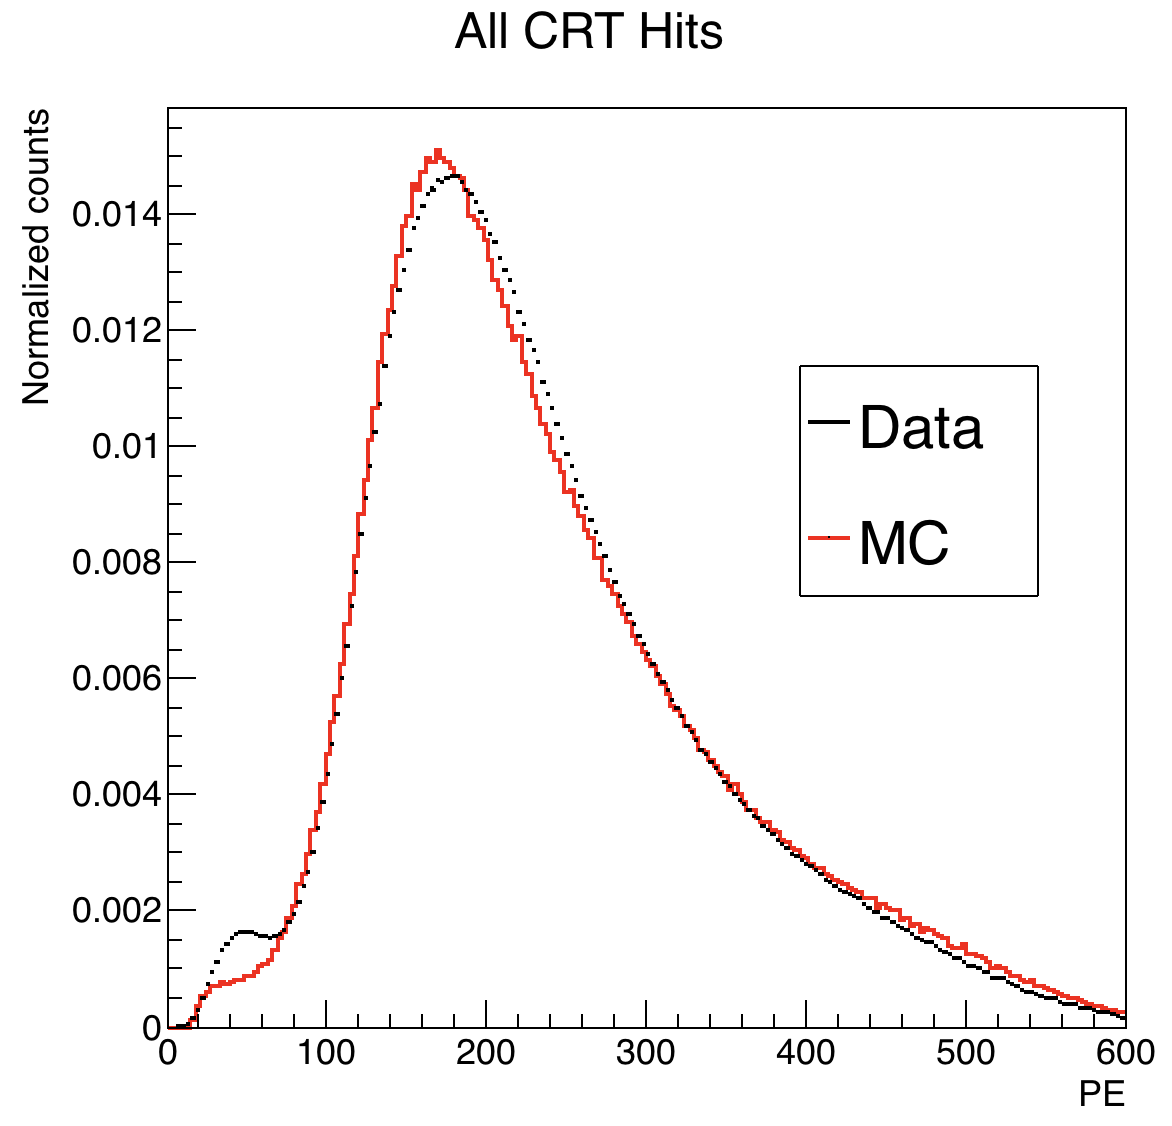
\includegraphics[scale=0.35]{images/CRTPENoCut}
\caption{PE distribution for CRT hits for data (black) and simulation (red). The distributions are area normalized.}
\label{fig:CRTPe}
\end{figure}



\subsection{Distance Tagger}\label{sec:DistCuts}
The scope of the CRT Distance Tagger is to reduce the number of events where cosmic ray activity in the detector is reconstructed as a neutrino interaction. We work under the assumption that most of the charged particles produced in a $\nu_e$ interaction should not deposit energy in any CRT module. 
%It should be noted that  when performing a CRT Hit to track association, we require that the TPC track length is at least 20 cm.  
In principle, extremely few tracks associated with the $\nu_e$ interaction products should be associated to CRT hits. On the contrary, cosmic rays wrongly associated to the neutrino vertex can leave a hit in the CRT, as well as  $\nu_\mu$ CC interactions with uncontained  muons.

The CRT Distance Tagger requires the presence of a reconstructed neutrino vertex.  We choose the pandora workflow to benchmark the performances of the CRT cuts in a electron neutrino search. The CRT cuts are easily exportable to different workflows, but in this work, we implemented the CRT Veto and CRT Distance Tagger within the pandora preselection stage. The evaluation of the pandora performances in electron neutrino searches is beyond the scope if this work: albeit wildly used, the pandora toolkit is still under development. Thus, we draw no conclusions regarding this toolkit, we disentangle the CRT  and pandora effects when possible and we present a performance assessment relative to this toolkit.\\

Before diving into the CRT Distance Tagger definition, we will spend a few words to describe both the CRT hit to TPC track matching and the relevant information provided by the pandora neutrino reconstruction. For the matching, we consider all CRT hits with signal $>$ 70 PE  and tracks longer than 20 cm. We then test every possible CRT Hit - TPC track combination as follows: 
\begin{itemize}
\item[1.] we assume the ionization electrons for the track started drifting at the time of the CRT hit, so we move the track in the drift direction according to the CRT hit time, 
\item [2.] we first correct the track for space charge effects and then project it towards the CRT plane containing the hit,
\item [3.] we calculate the distance of closest approach for the projected track and the CRT hit,
\item [4.] if the minimum distance is less than 40 cm for CRT hits in the top panel or less than 25 cm for  for CRT hits in the other panels, a match is found,
\item[5]if more than one match is found for a given track, the match with the smallest distance of closest approach is chosen. 
\end{itemize}

When a match is found, an association between the TPC track and the CRT hit is stored in the event. The track object is not modified, i.e. its position in the drift direction remains the original position, just more information about the track is added. Details of the matching algorithm will be documented  in a future technote.


Pandora reconstructs at most one neutrino interaction per event. Under the neutrino hypothesis, the reconstructed vertex position is given in three dimensions assuming that the ionization drift start time is the time of the flash which triggered the event. All the tracks associated to the neutrino event are reconstructed under this time hypothesis. 

The CRT Distance Tagger checks the minimum distance between the reconstructed vertex and each track associated with a CRT hit. At this time, we do now apply any space charge correction when calculating this distance.  If the minimum distance is less than 14 cm, the event is rejected. An example event tagged by this cut is shown in Figure~\ref{fig:crtdist00}. More such examples are in Appendix~\ref{app:crttagger}.

\begin{figure}[h!]
\centering
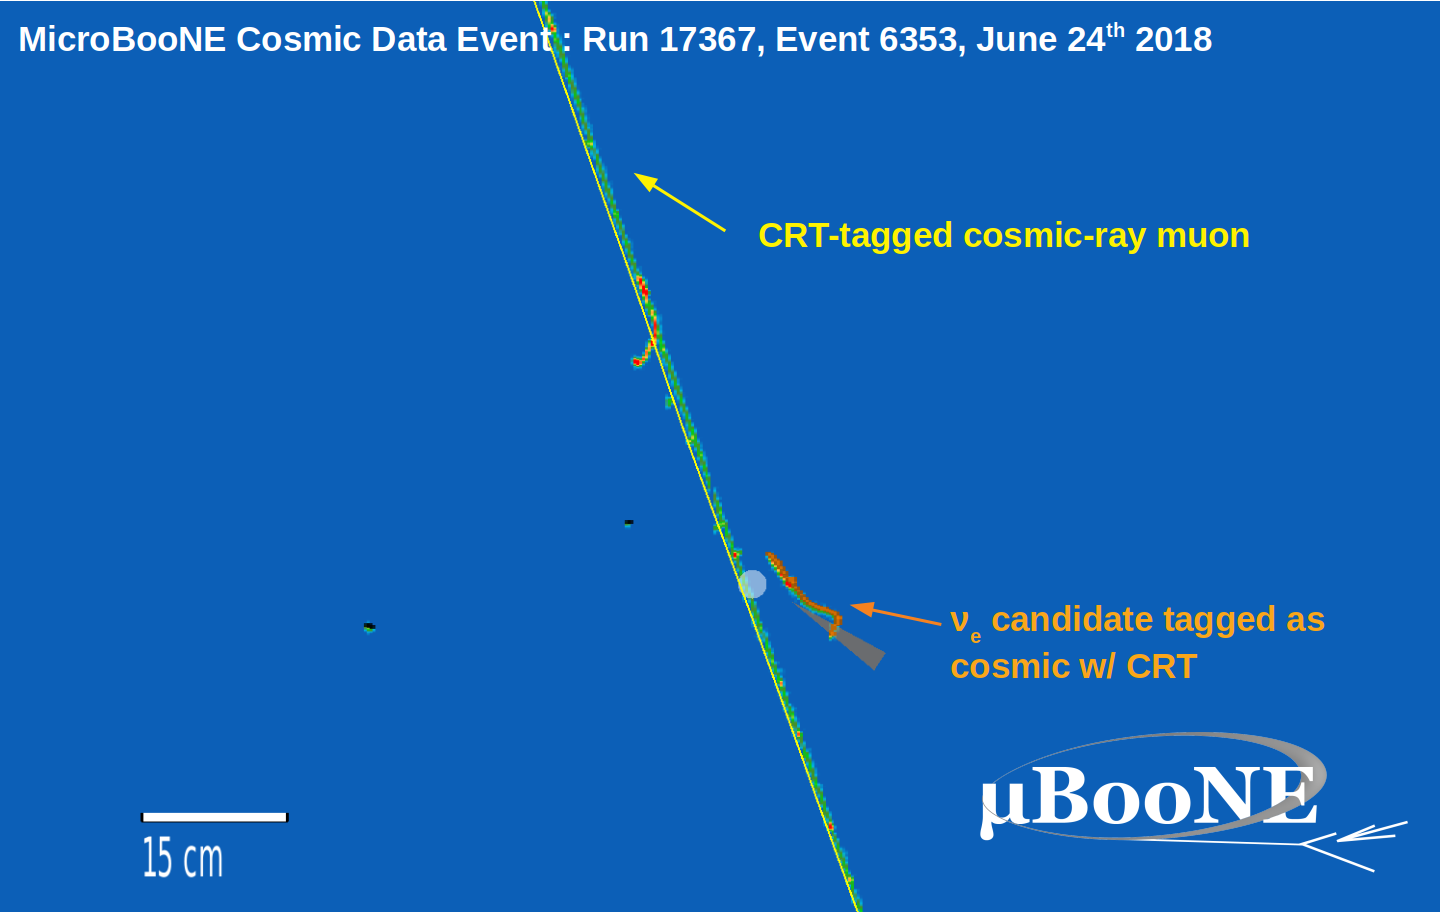
\includegraphics[width=0.9\textwidth]{images/crttagger_01.png}
\caption{Example $\nu_e$ candidate tagged as cosmic thanks to the CRT distance tagger. From the event one can see that the reconstructed EM shower is associated to EM activity associated to the incoming muon.}
\label{fig:crtdist00}
\end{figure}


\newpage
\section{Rejection Power and Signal Efficiency}\label{sec:RejectionAndEff}

Table \ref{tab:PS} lists all the cuts in the order they are applied in what we consider the neutrino preselection stage for this work. The CRT Veto is applied to the events passing the optical filter; the pandora neutrino reconstruction is then applied. No requirement on the neutrino nature is applied at this stage: the pandora reconstructed neutrino can be either a $\nu_e$ or a $\nu_\mu$. The final stage of the preselection is the CRT Distance tagger. 
We are reporting here the passing rates for each cut applied to three different samples:  BNB External,  BNB Run 3 (open 1e19) and  $\nu_e$ Overlay. For each sample, Table \ref{tab:PS} shows the number of events passing a given cut and the  passing rate relative to the previous stage; the total passing rate without CRT cuts and with CRT cuts is shown in the last two rows.

The interpretation of the effect of the CRT cuts on the BNB External is straightforward. Since no neutrinos are present in the BNB external sample, all events that pass a selection are to be considered background.  The rejection power of cosmic background is 79\% without the use of CRT information and increases to 94\% with the use of the CRT information.

The interpretation of the effect of the CRT cuts on the $\nu_e$ overlay sample is more complex and needs to be broken down into the effect of the CRT Veto and the CRT Distance cut separately.  
As a preamble, we should note that we require that each event in our overlay sample contains an electron neutrino whose interaction is generated in the TPC fiducial volume;  the fiducial volume is defined as follows (\textcolor{red}{LOOK for this dimensions}). No requirement is set on the containment of the charge particles produced in the interaction. Given this premise, the interpretation of the effect of the CRT Veto is, again, straightforward. Since all events include a $\nu_e$ interaction in the sample, all events rejected by the CRT Veto are to be considered an inefficiency.  Thus, the CRT Veto efficiency on electron neutrinos is overall 95\%. Figure \ref{fig:VetoE} shows the CRT Veto efficiency as a function of the true neutrino energy for true neutrino energies smaller than 2 GeV;  for true neutrino energies smaller than 700 MeV, the CRT Veto efficiency is greater than 96.5\%. 

Understanding the signal efficiency for the CRT Distance Tagger is more complicated, since the effect of the tagger is coupled with the identification of the vertex by the pandora framework. The last column of  Table \ref{tab:PS} shows a 7\% event reduction when applying the CRT Distance cut to the identified pandora neutrino vertex. However, there is no guarantee that pandora identifies the true neutrino activity: we just know a neutrino was reconstructed in the event.
If we want to understand the efficiency of the CRT Distance Tagger on the $\nu_e$ sample, we need to require that pandora identifies correctly the true neutrino vertex. We crudely check for truth matching by requiring that the distance between the true neutrino vertex and the reconstructed neutrino vertex is less than 14 cm: these events should not be cut by CRT Distance Tagger, they are legitimate signal events that we use as denominator to calculate the CRT Distance Tagger efficiency on the $\nu_e$ sample.  Under this signal definition, Figure \ref{fig:DistanceE} shows the CRT Distance Tagger efficiency as a function of the true neutrino energy for true neutrino energies smaller than 2 GeV;  for true neutrino energies smaller than 700 MeV, the CRT Veto efficiency is greater than 97.5\%. Using the same truth matching definition, we can now estimate the rejection power of CRT Distance Tagger for the cases where a true $\nu_e$ is generated in the event, but pandora mis-identifies cosmic activities as the neutrino interaction. For this study, we select events such that the distance between the true neutrino vertex and the reconstructed neutrino vertex is greater than 14 cm: for simplicity we flag all these events as background and we call this sample ``mis-ID $\nu$" sample. We then apply the CRT Distance cut. Unsurprisingly, 19\% percent of mis-identified neutrino interactions are removed by the CRT Distance tagger in the ``mis-ID $\nu$" sample; this is the same rejection power of the CRT Distance Cut on the BNB External. Since the CRT Distance Tagger cuts the same type of pandora misidentification in both BNB External and ``mis-ID $\nu$" samples, the same rejection power is expected.



\begin{table}[h]
\begin{tabular}{ c || c | c || c | c || c | c || }
\cline{2-7}
                                            & \multicolumn{2}{c||}{BNB External} & \multicolumn{2}{c||}{BNB Run 3 1e19} & \multicolumn{2}{c||}{$\nu_e$ overlay} \\ \cline{2-7} 
                                            & N evts        & Relative PS       & N evts         & Relative PS        & N evts       & Relative PS       \\ \hline
\multicolumn{1}{|l||}{Common Optical Filter}  & 56435         &                   & 35050          &                    & 150384       &                   \\ \hline
\multicolumn{1}{|l||}{CRT Veto}                       & 33330         & 59\%          & 22040          & 63\%               & 143227       & 95\%              \\ \hline
\multicolumn{1}{|l||}{Pandora Reco Neutrino} & 4587          & 14\%           & 5576           & 25\%              & 122390       & 85\%              \\ \hline
\multicolumn{1}{|l||}{CRT Distance}                & 3730          & 81\%            & 4861           & 87\%              & 114123       & 93\% ($>$96\%)              \\ \hline \hline 
\multicolumn{1}{|l||}{Total Passing Rate w/o CRT}    &         \multicolumn{2}{c||}{ 21\%}    &   \multicolumn{2}{c||}{28\%}  & \multicolumn{2}{c||}{85\%}\\ \hline
\multicolumn{1}{|l||}{Total Passing Rate w/ CRT}       &                 \multicolumn{2}{c||}{6\%}      & \multicolumn{2}{c||}{14\%}     &  \multicolumn{2}{c||}{76\% }   \\ \hline
\end{tabular}
\caption{Passing rates for neutrino preselection on BNB External, BNB and $\nu_e$ overlay Samples.}
\label{tab:PS}
\end{table}


\begin{figure}[h!]
\centering
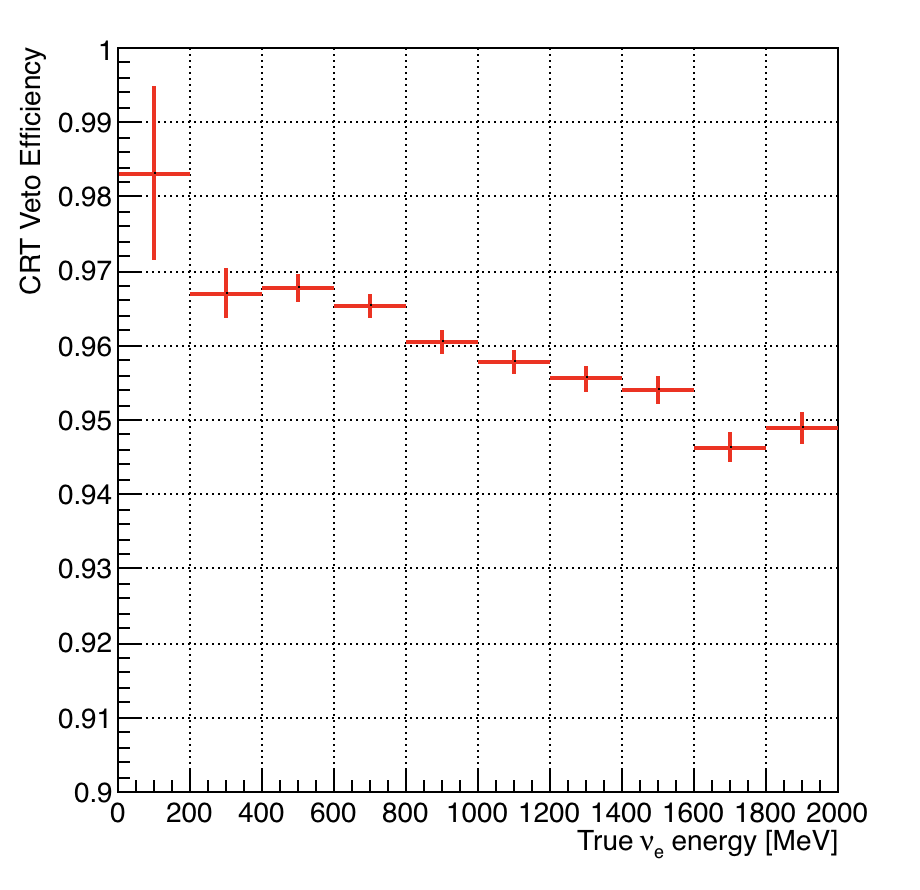
\includegraphics[scale=0.4]{images/CRTVetoEfficiency}
\caption{CRT Veto efficiency as a function of true neutrino energy in the low energy region.}
\label{fig:VetoE}
\end{figure}

\begin{figure}[h!]
\centering
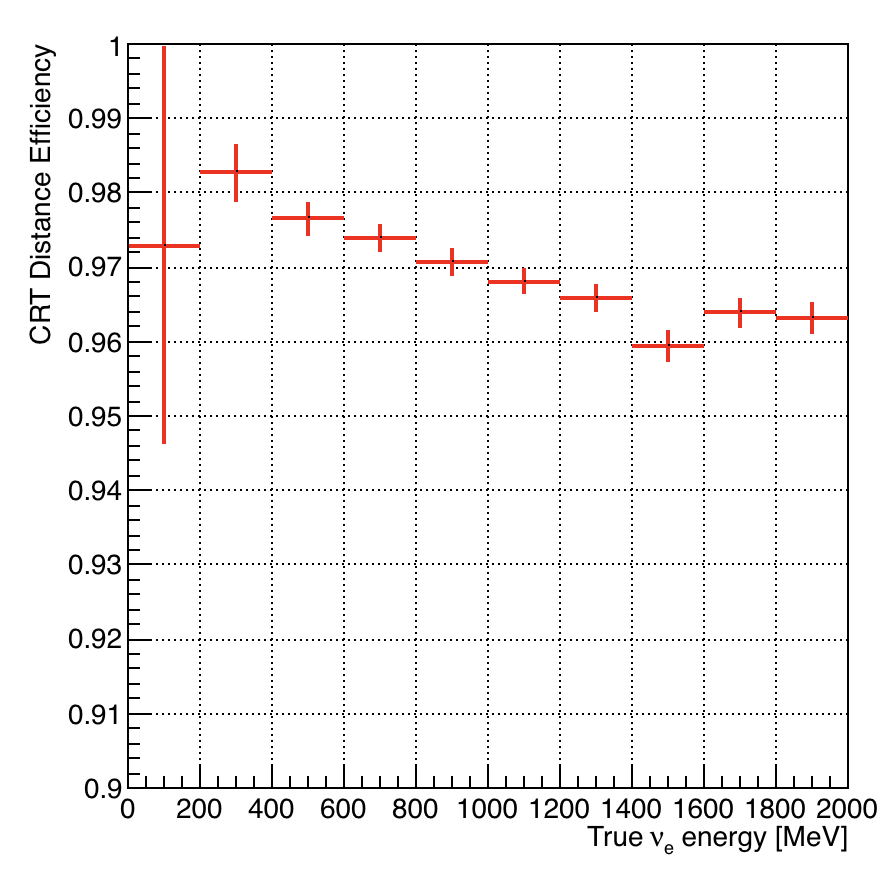
\includegraphics[scale=0.4]{images/CRTDistanceEfficiency}
\caption{CRT Distance Tagger efficiency as a function of true neutrino energy in the low energy region.}
\label{fig:DistanceE}
\end{figure}

\newpage
\section{Comparison of Cutflow Significance}\label{sec:Significance}
In the previous section, our preselection had no $\nu_e$ specific requirement. This was to disentangle the  effects of the CRT from the pandora reconstruction as much as possible. If we want to understand the impact of the CRT on the $\nu_e$ preselection, however, we need to require that pandora identifies a $\nu_e$ in the event.  This is done by imposing that the neutrino candidate identified by pandora have the dominant particle (by total number of hits) in the interaction be associated with a reconstructed shower. For the purpose of this work this is a crude but effective $\nu_e$ preselection.
Table \ref{tab:PSNue} shows the preselection passing rates adding the requirement of $\nu_e$ identification without and with the use of CRT information on the BNB External,  BNB Run 3 (open 1e19) and  $\nu_e$ Overlay samples. 


\begin{table}[h]
\begin{tabular}{ c || c | c || c | c || c | c || }
\cline{2-7}
                                            & \multicolumn{2}{c||}{BNB External} & \multicolumn{2}{c||}{BNB Run 3 1e19} & \multicolumn{2}{c||}{$\nu_e$ overlay} \\ \cline{1-7} 
\multicolumn{1}{|l||}{Total Passing Rate w/o CRT}    &         \multicolumn{2}{c||}{ 1.2\%}    &   \multicolumn{2}{c||}{1.7\%}  & \multicolumn{2}{c||}{63.3\%}\\ \hline
\multicolumn{1}{|l||}{Total Passing Rate w/ CRT}       &                 \multicolumn{2}{c||}{0.4\%}      & \multicolumn{2}{c||}{0.98\%}     &  \multicolumn{2}{c||}{58.6\% }   \\ \hline
\end{tabular}
\caption{Passing rates for $\nu_e$ preselection on BNB External, BNB and $\nu_e$ overlay Samples.}
\label{tab:PSNue}
\end{table}


Since a $\nu_e$ was found in the event, we can now compare the effect of the CRT in relation to the reconstructed energy of the leading shower in the event.
Figure \ref{fig:SelVsShowerE} shows the effect of the $\nu_e$ preselection on BNB external (black) and on BNB  (blue) data normalized to 0.8E19 POT as a function of the reconstructed leading shower energy; on the left we see the effect of the preselection without the use of the CRT cuts, while on the right we see the effect of the preselection including the  CRT cuts. The statistics for shower energy bins greater than 1 GeV is extremely limited (and far from the range relevant to the low energy excess search); we will discard those bins in further considerations. 

We can now calculate the significance of the preselection as a function of the leading shower energy for in the two cases.
We define the significance as the ratio of signal over background (S/B). We estimate the background as the number of events passing the preselection in the BNB external sample (EXT); we estimate the signal as the number of events passing the preselection in the BNB samples minus the number of events passing the preselection in the BNB external sample (BNB - EXT). Figure \ref{fig:Significance} on the left shows the S/B ratio as a function of the reconstructed shower energy for the preselection using CRT information (red) and without using CRT information (blue). 
Figure \ref{fig:Significance} on the right shows the percentage of signal in the BNB (i.e. S/(S+B)) as a function of the reconstructed shower energy for the preselection using CRT information (red) and without using CRT information (blue). The error bars are calculated via a conservative Feldman-Cousins technique where we estimate that the measured value lies between the error bars 68\% of the times. Even with low statistics, the improvements with the use of the CRT are significant. In the lower energy bins, the preselection significance increases by a factor of 2 or more when using CRT information and the signal content goes from 50-65\% to 70-85\%.


\begin{figure}[h!]
\centering
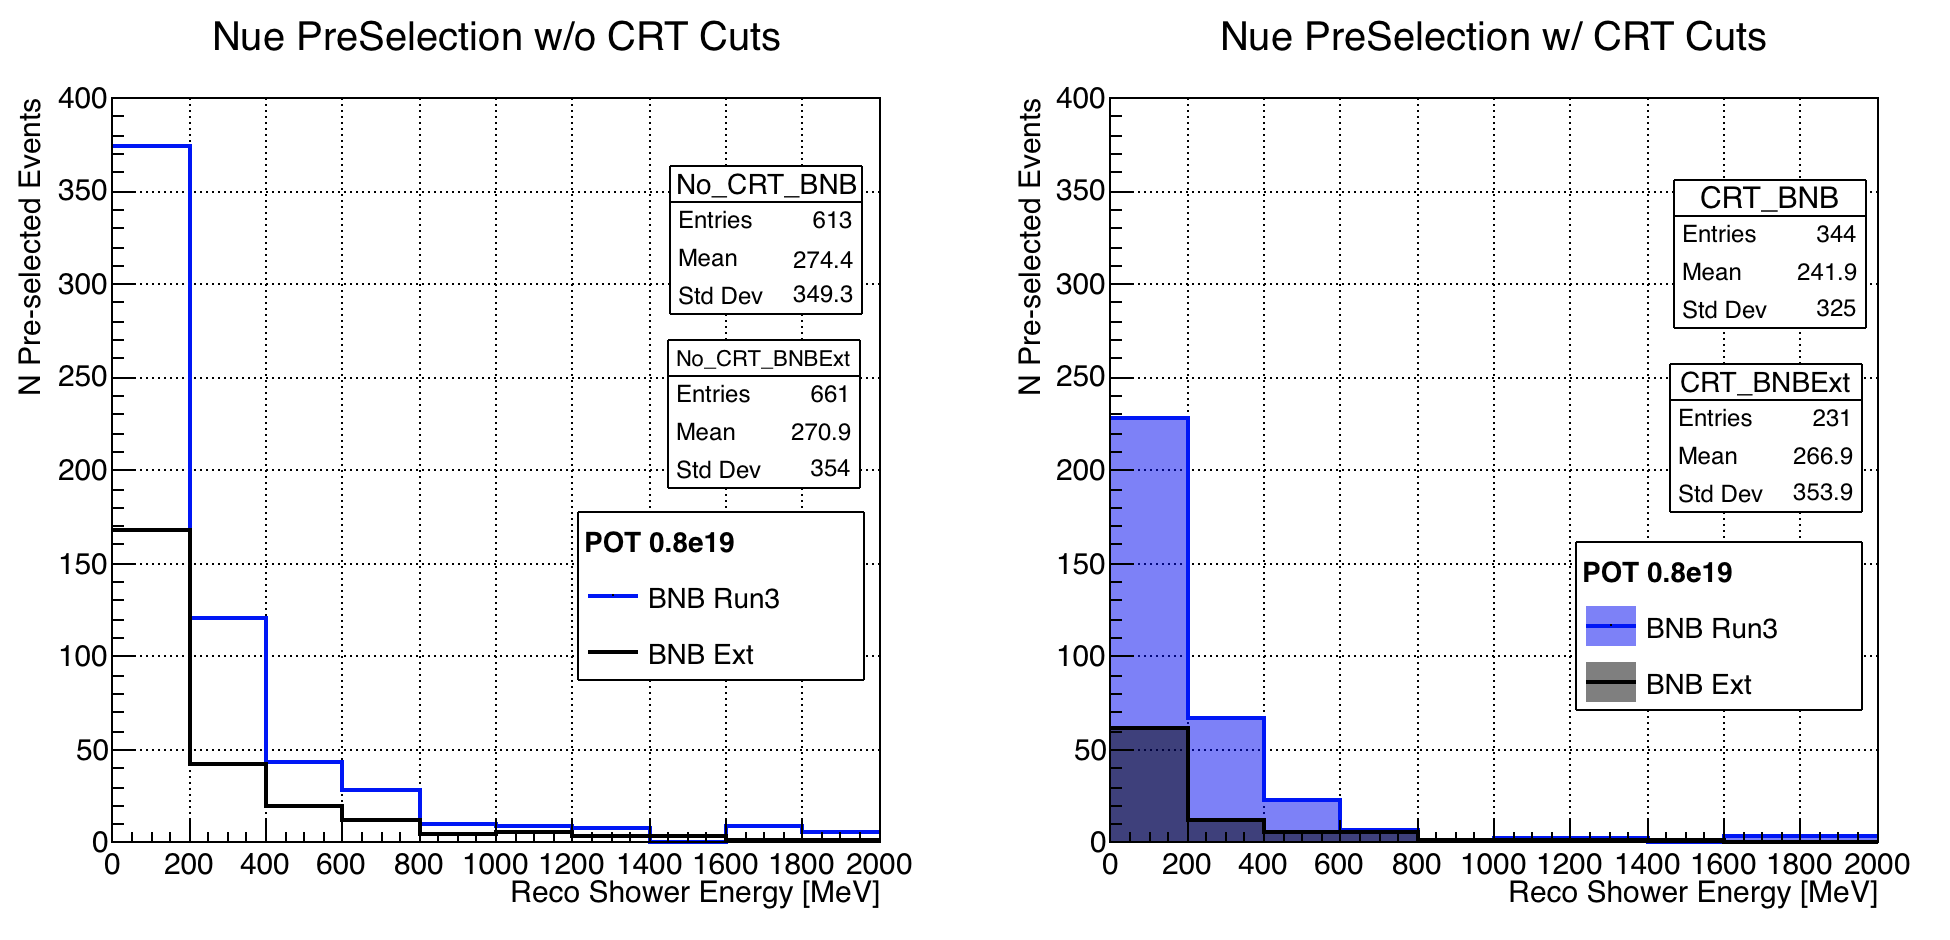
\includegraphics[scale=0.4]{images/Compare}
\caption{Events passing the $\nu_e$ preselection as a function of reconstructed leading shower energy for the BNB External sample (black) and the BNB sample (blue) normalized to 0.8E19 POT; the left figure shows the effect of the preselection without the CRT cuts, while the figure on the right shows  the effect of the preselection including the CRT cuts. }
\label{fig:SelVsShowerE}
\end{figure}

\begin{figure}[h!]
\centering
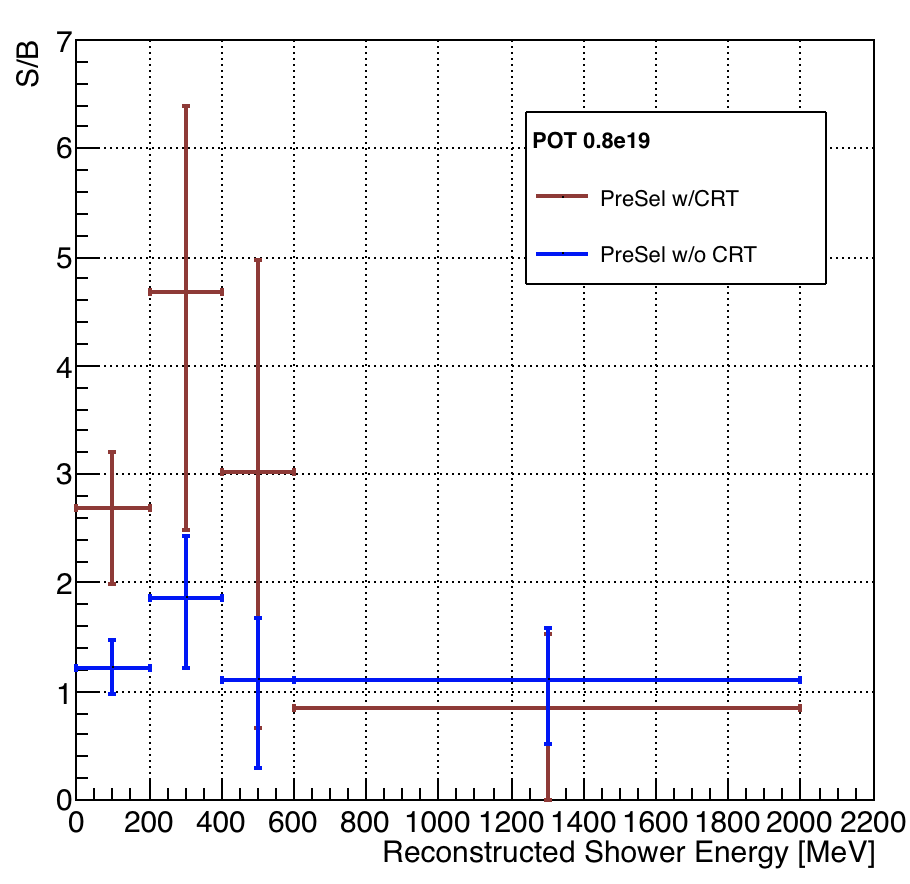
\includegraphics[scale=0.4]{images/SoverB}
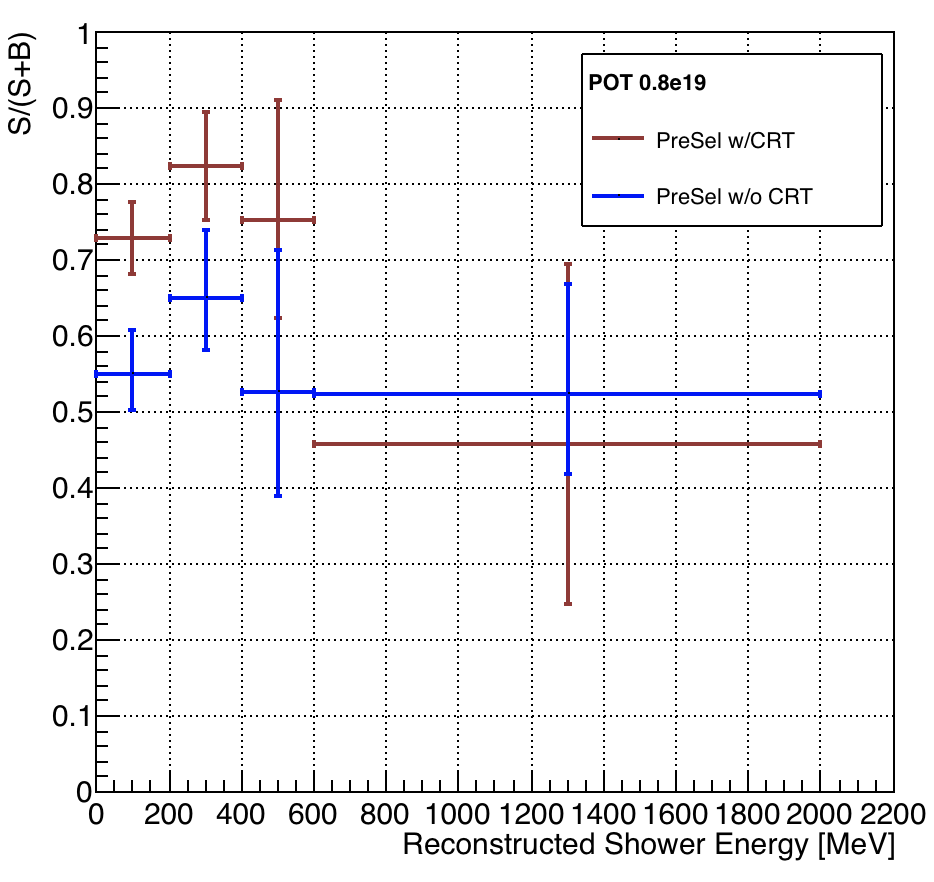
\includegraphics[scale=0.4]{images/SOverTot.png}
\caption{\textit{Left:} S/B for the preselection using CRT information (red) and without CRT information (blue). \textit{Right:} S/(S+B) for the preselection using CRT information (red) and without CRT information (blue).}
\label{fig:Significance}
\end{figure}

\section{Conclusions}\label{sec:Conclusions}
The MicroBooNE Cosmic Ray Tagger  (CRT) can be a powerful tool to reduce cosmic ray background in neutrino searches, especially if used at the early stages of neutrino selection (preselection). When used in physics analyses, it is important to study the stability of the CRT response and its impact to the analysis. We presented here a quick study of the CRT stability which proof that a) monitoring systems are in place at the level of the physics analysis and b) the CRT response is stable for the data period analysed.
We then proceeded to study the impact of the CRT on the preselection for $\nu_e$ searches. In particular, we studied the impact of the CRT Veto and CRT Distance Tagger on the BNB External, BNB and $\nu_e$ Overlay samples. ion as a function of the reconstructed leading shower energy. With the use of the CRT, the cosmics contribution in the preselectio
n decreases by factor of 3.5: the BNB External passing rate goes from 21\% to 6\%. By applying the pandora $\nu_e$ identification, we studies the significance of the preselection with and without the use of CRT informat and the significance increases by at least a factor of two in the low energy bins.

\newpage

\appendix

\section{CRT Track-Tagger Event Displays}

The images below show example events where a $\nu_e$ candidate was tagged by the CRT distance tagger.

\begin{figure}[h!]
\centering
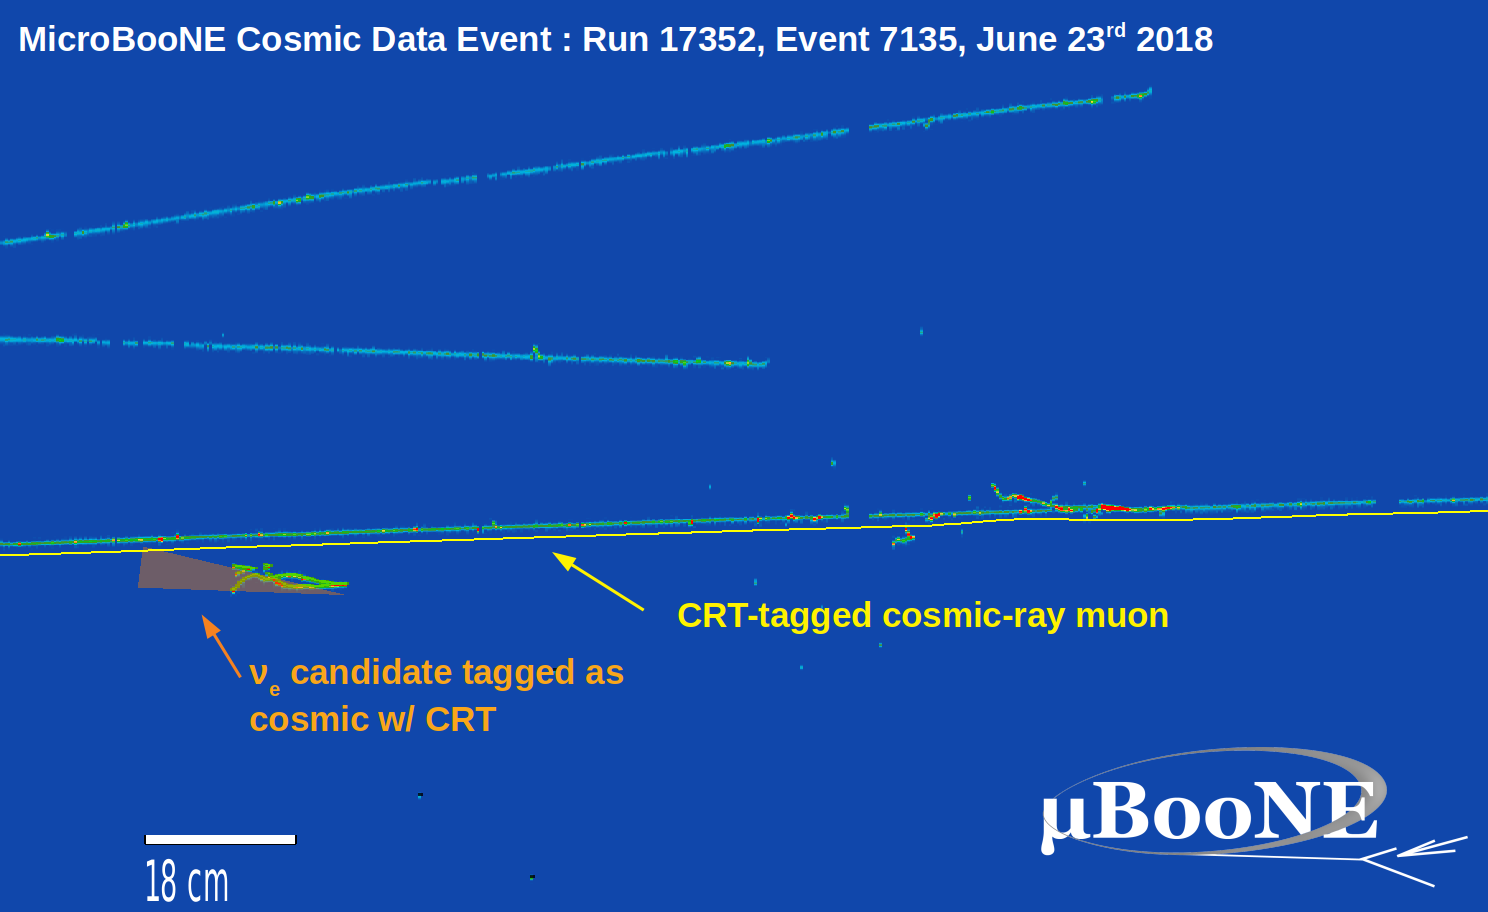
\includegraphics[width=0.9\textwidth]{images/crttagger_00.png}
\caption{Example $\nu_e$ candidate tagged as cosmic thanks to the CRT distance tagger. From the event one can see that the reconstructed EM shower is associated to EM activity associated to the incoming muon.}
\label{fig:crtdist00}
\end{figure}


\begin{figure}[h!]
\centering
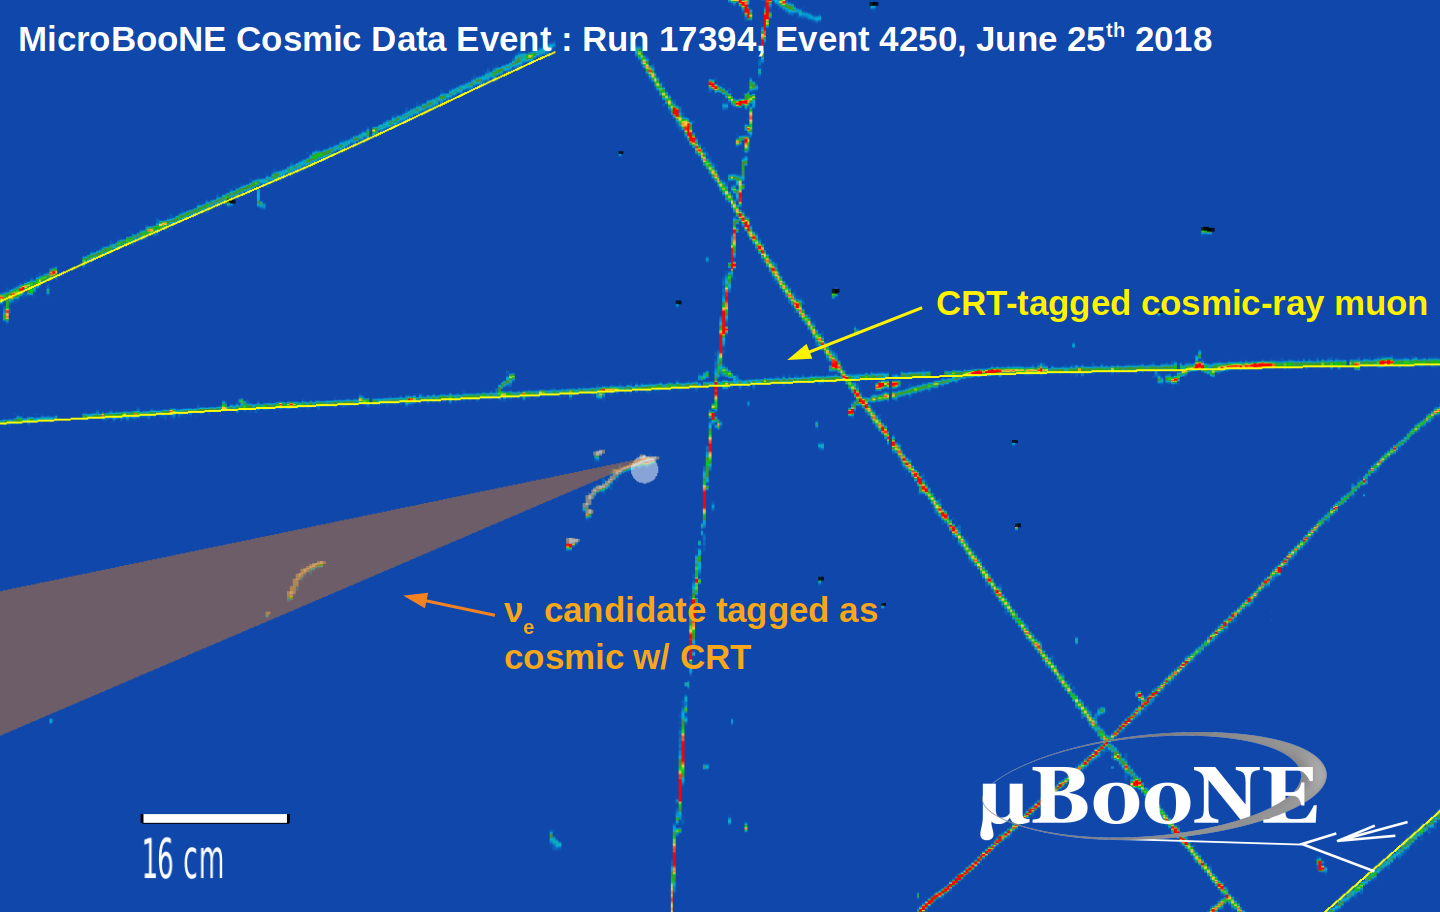
\includegraphics[width=0.9\textwidth]{images/crttagger_02.png}
\caption{Example $\nu_e$ candidate tagged as cosmic thanks to the CRT distance tagger. From the event one can see that the reconstructed EM shower is associated to EM activity associated to the incoming muon.}
\label{fig:crtdist00}
\end{figure}

\begin{figure}[h!]
\centering
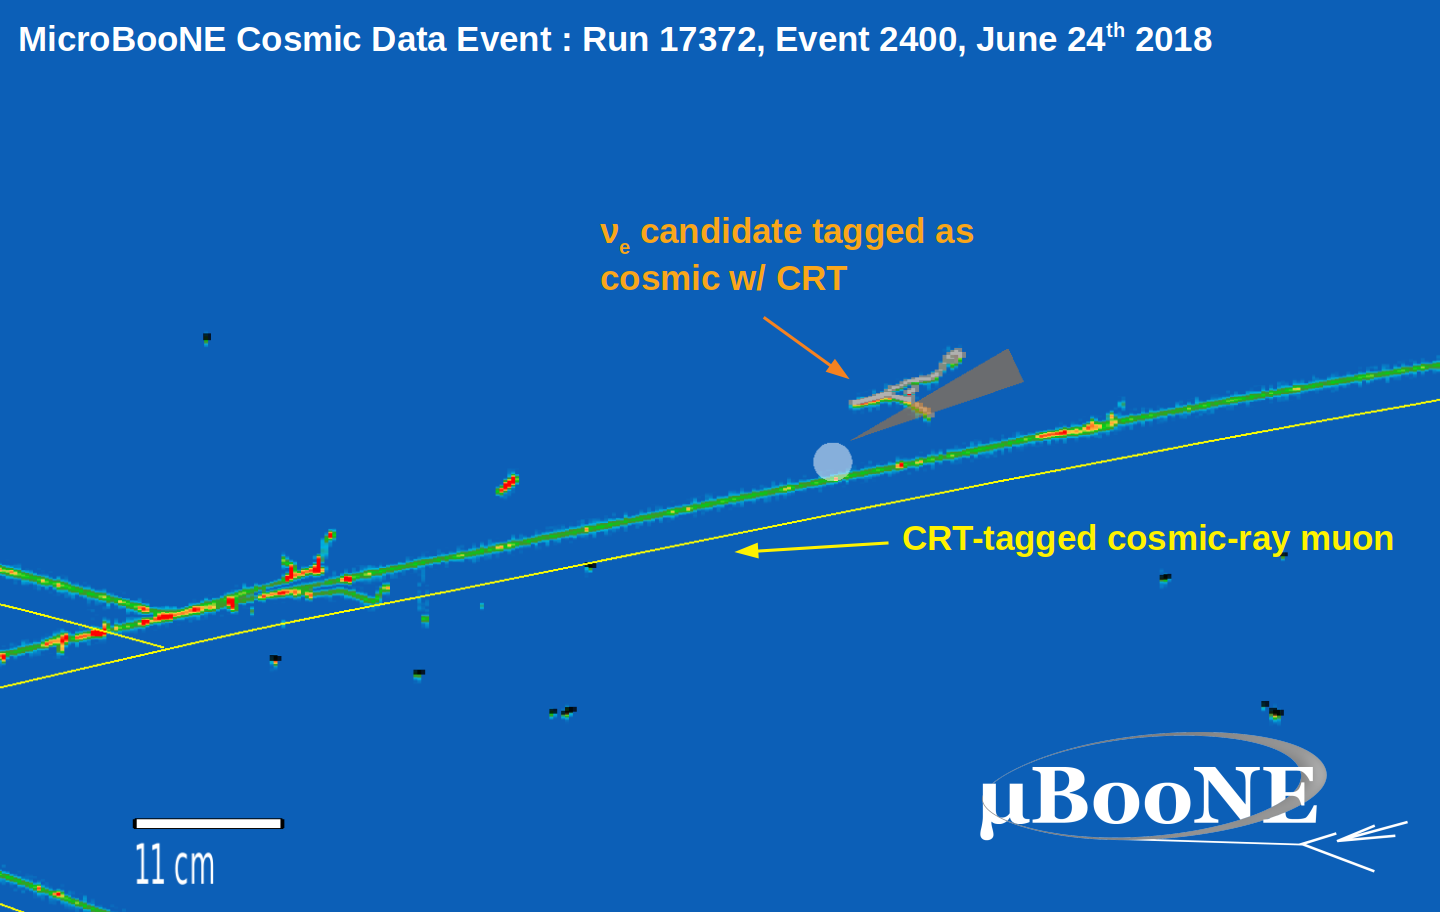
\includegraphics[width=0.9\textwidth]{images/crttagger_03.png}
\caption{Example $\nu_e$ candidate tagged as cosmic thanks to the CRT distance tagger. From the event one can see that the reconstructed EM shower is associated to EM activity associated to the incoming muon.}
\label{fig:crtdist00}
\end{figure}
